コードの設計、開発環境のセットアップ、スクショ、工夫したところ
ここでは開発したアプリケーションに関する工夫を説明する.

\subsection{アプリケーションの開発環境}
 webアプリケーション開発にはjavascriptのwebフレームワークであるNode.jsを用いた.Node.jsのパッケージであるexpressとnanoを用いた.expressはwebフレームワークで、nanoはCouchDBのためのドライバである.

\begin{table}[htb]
	\begin{tabular}{|l|c|r|r|}\hline
	導入ソフト & ヴァージョン \\ \hline \hline
	Node.js & 0.12.6 \\ \hline
	Express & 4.12.1 \\ \hline
	Passport & 未定 \\ \hline
	\end{tabular}
\end{table}


\subsection{データベースの設計}
	CouchDBにss-mixの仕様書から引っ張ってきたデータ格納方法およびデータ定義\cite{bibi1}に基づいてデータを格納する.
	\begin{figure}[htbp]
		\begin{center}
			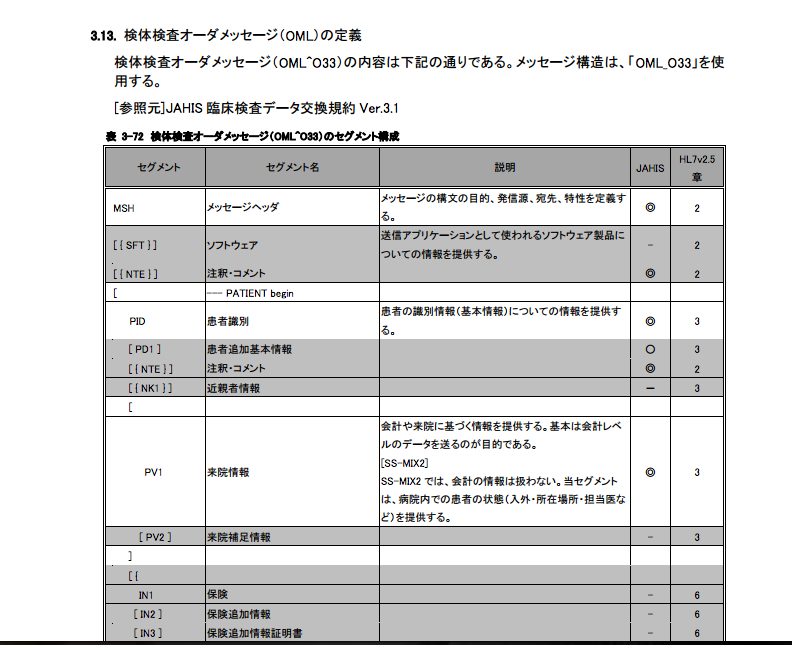
\includegraphics[width=5cm, bb=0 0 645 790]{ss-mix_sample.png} %よこたて
		\end{center}
		\caption{データ定義}
		\label{ss-mix_sample}
	\end{figure}

	\begin{figure}[htbp]
		\begin{center}
			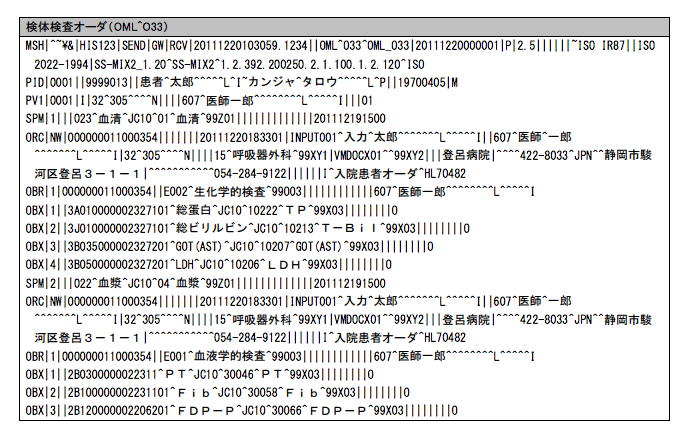
\includegraphics[width=5cm, bb=0 0 437 688]{ss-mix_sampledata.png}
		\end{center}
		\caption{データサンプル}
		\label{ss-mix_sampledata}
	\end{figure}

\subsection{アプリケーションの設計}


\subsection{アプリケーションの機能}
 医療情報を収集するNoSQLデータベースシステム.UIとしてWebアプリを用意し、医療関係者、薬剤師、患者の3者に対して、情報を扱いやすいようにした.

	\subsubsection{患者情報閲覧}
		必要な人に必要な情報が見えるヴューを用意する.
		血圧とか、血糖とか、項目を指定したらその項目の数値を
		異なるフォーマットによって投入されてるドキュメントからひっぱってきて表示する.

	\subsubsection{共有の許可,権限}
		患者が情報共有する医療関係者を選択する.

	\subsubsection{データベースの利用}
		1診療1ドキュメント
		どうやってCouchからデータを引っ張ってきているか.
		患者のドキュメントを検索してからデータを取得.

	\subsubsection{データの投入方法}
		 患者,医療関係者からの投入を受け付ける.
		 ファイルを指定してpostで送信してる.
